\subsection{LOCALLY COMPACT σ-COMPACT SPACES}

DEFINITION 5. A locally compact space X is said to be σ-compact or countable at infinity if it is a countable union of compact subsets.

Examples. 1) A discrete space is \(\sigma\) -compact if and only if it is countable. *2) The real line \(\mathbf{R}\) is locally compact and \(\sigma\) -compact, since it is the union of the compact intervals \([-n, +n]\) for \(n \in \mathbb{N}\) . *

\pandocbounded{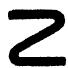
\includegraphics[keepaspectratio]{images/part001_9ca68205.jpg}}

Remark. A Hausdorff space can be a countable union of compact subspaces without being locally compact. * An example is Hilbert space with the weak topology, as we shall show in a later volume.

PROPOSITION 15. If X is a locally compact \(\sigma\) -compact space, there is a sequence \((\mathbf{U}_n)\) of relatively compact open subsets of X which cover X, such that \(\overline{\mathbf{U}}_n \subset \mathbf{U}_{n+1}\) for each \(n\) .

Let X be the union of a sequence \((\mathbf{K}_{n})\) of compact sets. Let \(U_{1}\) be a relatively compact open neighbourhood of \(K_{1}\) (no. 7, Proposition 10) and define \(U_{n}\) inductively for n \textgreater{} 1 to be a relatively compact open neighbourhood of \(\overline{U}_{n-1} \in K_{n}\) (no. 3, Proposition 5; no. 7, Proposition 10). The sequence \((\mathbf{U}_{n})\) clearly has the required properties.

COROLLARY I. With the notation of Proposition 15, every compact subset K of X is contained in some \(U_{n}\) .

For K can be covered by a finite number of the \(U_{k}\) , by axiom (C'\,').

COROLLARY 2. Let X be a locally compact space and let X' be the compact space obtained by adjoining a point at infinity ω to X (no. 8). Then X is σ-compact if and only if the point ω has a countable fundamental system of neighbourhoods in X'.

If X is σ-compact we can construct a sequence of subsets \(U_{n}\) of X as in Proposition 15, and the neighbourhoods \(X^{\prime}-\overline{U}_{n}\) of \(\omega\) in \(X^{\prime}\) form a fundamental system of neighbourhoods of \(\omega\) by reason of Corollary 1. The converse follows from the fact that the complements of open neighbourhoods of \(\omega\) are compact subsets of X.

Clearly every closed subspace of a locally compact \(\sigma\) -compact space is locally compact and \(\sigma\) -compact. Likewise any finite product of locally compact \(\sigma\) -compact spaces is locally compact and \(\sigma\) -compact.

Notice, however, that an open subspace of a compact space need not be \(\sigma\) -compact, as Alexandroff's theorem (no. 8, Theorem 4) shows.

